\usetikzlibrary{arrows.meta}
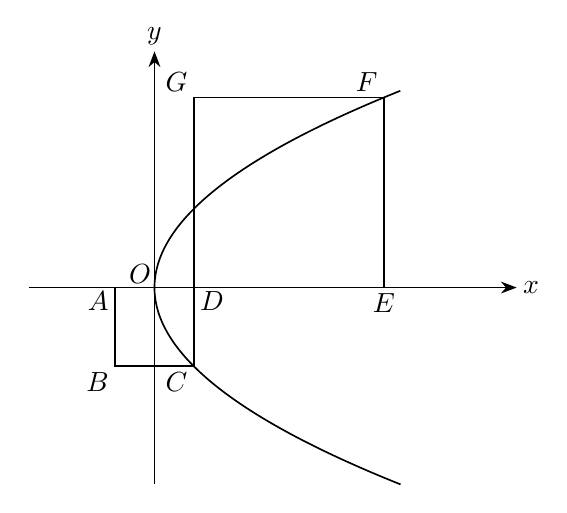
\begin{tikzpicture}[x=1cm,y=1cm,line width=.6pt,font=\normalsize,>=Stealth]
\coordinate (O) at (0,0);
\coordinate (A) at (-0.5,0);
\coordinate (D) at (0.5,0);
\coordinate (B) at (-0.5,-1);
\coordinate (C) at (0.5,-1);
\coordinate (E) at (2.9142135624,0);
\coordinate (G) at (0.5,2.4142135624);
\coordinate (F) at (2.9142135624,2.4142135624);
\draw[->] (-1.6,0) -- (4.6,0) node[right,inner sep=0pt,xshift=2pt] {$x$};
\draw[->] (0,-2.5) -- (0,3.0) node[above,inner sep=0pt,yshift=2pt] {$y$};
\draw (A)--(B)--(C)--(D)--(G)--(F)--(E);
\draw[domain=-2.5:2.5,samples=201] plot ({\x*\x/2},\x);
\node[above left,inner sep=0pt,xshift=-1pt,yshift=1pt] at (O) {$O$};
\node[below left,inner sep=0pt,xshift=-2pt,yshift=-1pt] at (A) {$A$};
\node[below right,inner sep=0pt,xshift=2pt,yshift=-1pt] at (D) {$D$};
\node[below,inner sep=0pt,yshift=-2pt] at (E) {$E$};
\node[below left,inner sep=0pt,xshift=-2pt,yshift=-2pt] at (B) {$B$};
\node[below left,inner sep=0pt,xshift=-2pt,yshift=-2pt] at (C) {$C$};
\node[above left,inner sep=0pt,xshift=-2pt,yshift=2pt] at (G) {$G$};
\node[above left,inner sep=0pt,xshift=-2pt,yshift=2pt] at (F) {$F$};
\end{tikzpicture}
